\documentclass[12pt]{article}\usepackage[]{graphicx}\usepackage[]{color}
%% maxwidth is the original width if it is less than linewidth
%% otherwise use linewidth (to make sure the graphics do not exceed the margin)
\makeatletter
\def\maxwidth{ %
  \ifdim\Gin@nat@width>\linewidth
    \linewidth
  \else
    \Gin@nat@width
  \fi
}
\makeatother

\definecolor{fgcolor}{rgb}{0.345, 0.345, 0.345}
\newcommand{\hlnum}[1]{\textcolor[rgb]{0.686,0.059,0.569}{#1}}%
\newcommand{\hlstr}[1]{\textcolor[rgb]{0.192,0.494,0.8}{#1}}%
\newcommand{\hlcom}[1]{\textcolor[rgb]{0.678,0.584,0.686}{\textit{#1}}}%
\newcommand{\hlopt}[1]{\textcolor[rgb]{0,0,0}{#1}}%
\newcommand{\hlstd}[1]{\textcolor[rgb]{0.345,0.345,0.345}{#1}}%
\newcommand{\hlkwa}[1]{\textcolor[rgb]{0.161,0.373,0.58}{\textbf{#1}}}%
\newcommand{\hlkwb}[1]{\textcolor[rgb]{0.69,0.353,0.396}{#1}}%
\newcommand{\hlkwc}[1]{\textcolor[rgb]{0.333,0.667,0.333}{#1}}%
\newcommand{\hlkwd}[1]{\textcolor[rgb]{0.737,0.353,0.396}{\textbf{#1}}}%
\let\hlipl\hlkwb

\usepackage{framed}
\makeatletter
\newenvironment{kframe}{%
 \def\at@end@of@kframe{}%
 \ifinner\ifhmode%
  \def\at@end@of@kframe{\end{minipage}}%
  \begin{minipage}{\columnwidth}%
 \fi\fi%
 \def\FrameCommand##1{\hskip\@totalleftmargin \hskip-\fboxsep
 \colorbox{shadecolor}{##1}\hskip-\fboxsep
     % There is no \\@totalrightmargin, so:
     \hskip-\linewidth \hskip-\@totalleftmargin \hskip\columnwidth}%
 \MakeFramed {\advance\hsize-\width
   \@totalleftmargin\z@ \linewidth\hsize
   \@setminipage}}%
 {\par\unskip\endMakeFramed%
 \at@end@of@kframe}
\makeatother

\definecolor{shadecolor}{rgb}{.97, .97, .97}
\definecolor{messagecolor}{rgb}{0, 0, 0}
\definecolor{warningcolor}{rgb}{1, 0, 1}
\definecolor{errorcolor}{rgb}{1, 0, 0}
\newenvironment{knitrout}{}{} % an empty environment to be redefined in TeX

\usepackage{alltt}

\usepackage{cmap}
\usepackage[unicode]{hyperref}
\usepackage[utf8]{inputenc}
\usepackage[T2A]{fontenc}
\usepackage[russian]{babel}
\usepackage{indentfirst}
\usepackage[left=2.5cm,right=1.5cm,top=2cm,bottom=2cm]{geometry}
\usepackage{fancyvrb}
\usepackage{float}
\IfFileExists{upquote.sty}{\usepackage{upquote}}{}
\begin{document}
\begin{center}
	Отчет по курсу СУБД, SQL и OLAP технологии \\* ИС-М16, Рябов Петр
\end{center}	

\tableofcontents
\newpage
\section*{Введение}
\addcontentsline{toc}{section}{Введение}
 % описать постановку задачи - какие группы и за какое время надо проанализировать
Требуется проанализировать успеваемость студентов групп бакалавриата специальности \textbf{<<Информационные системы и технологии>>} 2011-2013 года поступления за 2 и 3 семестр. То есть, группы ИС-Б11, Б12, Б13.
\section{SQL-запросы}
% привести запросы для получения списка групп и данных об оценках студентов

\begin{Verbatim}
//Извлекаем все группы по шаблону бакалавры ИС
SELECT * FROM sgroup WHERE shname LIKE 'ИС-Б__';

//Берем только их GID
SELECT gid FROM sgroup WHERE shname LIKE 'ИС-Б__';

//Извлекаем всех студентов из выбранных групп (Бакалавры ИС)
SELECT * FROM student WHERE gid IN (SELECT gid FROM sgroup WHERE shname LIKE 'ИС-Б__');

//Извлекаем информацию об успеваемости конкретного студента за 2-3 семестр
SELECT stid, discid, semnum, sum(ktmark) FROM studmark
    WHERE stid = '3844' AND (semnum >=2 AND semnum <=3)
    GROUP BY stid, discid, semnum;

//Полная информация об успеваемости студентов выбранных групп за 2-3 семестр
SELECT stid, semnum, discid, SUM(ktmark) FROM studmark
	WHERE stid IN (SELECT stid FROM student
		WHERE gid IN (SELECT gid FROM sgroup
			WHERE shname LIKE 'ИС-Б__')) 
	AND (semnum >=2 AND semnum <=3)
	GROUP BY stid, semnum, discid
	ORDER BY stid;
\end{Verbatim}

\begin{Verbatim}
//Полная информация об успеваемости + имена групп и дисциплин
===========================================================
SELECT g.shname, info.gid, info.stid, p.discname,
       info.discid, info.semnum, info.sum FROM (  
SELECT stid, discid, semnum, sum(ktmark) FROM studmark
	WHERE stid IN (SELECT stid FROM student
		WHERE gid IN (SELECT gid FROM sgroup
			WHERE shname LIKE 'ИС-Б__')) 
	AND (semnum >=2 AND semnum <=3)
	GROUP BY stid, discid, semnum
	ORDER BY stid
) info
JOIN predmet p ON p.discid = info.discid
JOIN (select gid, stid from student) s ON s.stid=info.stid
JOIN (select gid, shname from sgroup) g ON s.gid=g.gid;
\end{Verbatim}

\section{Загрузка данных в R}
Исходный код скрипта загрузки данных, с последующей их записью в CSV файл
\begin{knitrout}
\definecolor{shadecolor}{rgb}{0.969, 0.969, 0.969}\color{fgcolor}\begin{kframe}
\begin{alltt}
\hlkwd{library}\hlstd{(RPostgreSQL)}
\hlstd{drv} \hlkwb{=} \hlkwd{dbDriver}\hlstd{(}\hlstr{"PostgreSQL"}\hlstd{)}
\hlstd{con} \hlkwb{=} \hlkwd{dbConnect}\hlstd{(drv,} \hlkwc{dbname} \hlstd{=} \hlstr{"test"}\hlstd{,} \hlkwc{host} \hlstd{=} \hlstr{"127.0.0.1"}\hlstd{,}
                                \hlkwc{user} \hlstd{=} \hlstr{"test"}\hlstd{,} \hlkwc{password} \hlstd{=} \hlstr{"123"}\hlstd{)}

\hlstd{extractQuery} \hlkwb{<-}\hlstr{"SELECT g.shname, info.gid, info.stid, p.discname,info.discid,
info.semnum, info.sum FROM (  
SELECT stid, discid, semnum, sum(ktmark) FROM studmark
    WHERE stid IN (SELECT stid FROM student
        WHERE gid IN (SELECT gid FROM sgroup
            WHERE shname LIKE 'ИС-Б__')) 
    AND (semnum >=2 AND semnum <=3)
    GROUP BY stid, discid, semnum
    ORDER BY stid
) info
JOIN predmet p ON p.discid = info.discid
JOIN (select gid, stid from student) s ON s.stid=info.stid
JOIN (select gid, shname from sgroup) g ON s.gid=g.gid;"}

\hlstd{data} \hlkwb{<-} \hlkwd{dbGetQuery}\hlstd{(con, extractQuery)}
\hlkwd{write.csv}\hlstd{(data,} \hlkwc{file}\hlstd{=}\hlstr{"~/extractDataPR.csv"}\hlstd{,} \hlkwc{na}\hlstd{=}\hlstr{""}\hlstd{)}

\hlkwd{dbDisconnect}\hlstd{(con)}
\hlkwd{dbUnloadDriver}\hlstd{(drv)}
\end{alltt}
\end{kframe}
\end{knitrout}
Восстановление данных производится аналогично путем загрузки данных из CSV файла в dataframe.

\section{Анализ данных}
\subsection{Выбор групп и периода для анализа}
В качестве периода для анализа успеваемости был выбран 2 семестр, так как нет сведений оценок ИС-Б13 за 3 семестр. Первоначальным этапом анализа являлась кластеризация студентов по оценкам 2 семестра методом k-средних. Преобразование в широкую таблицу:

\begin{verbatim}
isB13sem2 <- dcast(cutGroup(333,2), stid ~ discid)
\end{verbatim}

 содержит N/A значение, более того в этой группе меньше всего студентов. Поэтому группа ИС-Б13 не кластеризуется.\newpage
 
\begin{knitrout}
\definecolor{shadecolor}{rgb}{0.969, 0.969, 0.969}\color{fgcolor}\begin{kframe}
\begin{alltt}
\hlkwd{library}\hlstd{(dplyr)}
\hlkwd{library}\hlstd{(ggplot2)}
\hlkwd{library}\hlstd{(reshape2)}

\hlstd{adata} \hlkwb{<-} \hlkwd{tbl_df}\hlstd{(}\hlkwd{read.csv}\hlstd{(}\hlkwc{file} \hlstd{=} \hlstr{"~/extractDataPR.csv"}\hlstd{)[ ,}\hlnum{2}\hlopt{:}\hlnum{8}\hlstd{])}

\hlstd{cutGroup} \hlkwb{<-} \hlkwa{function}\hlstd{(}\hlkwc{agid}\hlstd{,} \hlkwc{asem}\hlstd{) \{}
  \hlstd{g} \hlkwb{<-} \hlkwd{filter}\hlstd{(adata, gid} \hlopt{==} \hlstd{agid} \hlopt{&} \hlstd{semnum} \hlopt{==} \hlstd{asem)}
  \hlstd{cg} \hlkwb{<-} \hlstd{g[,}\hlkwd{c}\hlstd{(}\hlstr{"stid"}\hlstd{,} \hlstr{"discid"}\hlstd{,} \hlstr{"sum"}\hlstd{)]}
  \hlkwd{return}\hlstd{(cg)}
\hlstd{\}}
  \hlstd{B11} \hlkwb{<-} \hlkwd{cutGroup}\hlstd{(}\hlnum{222}\hlstd{,}\hlnum{2}\hlstd{)}
  \hlstd{B12} \hlkwb{<-} \hlkwd{cutGroup}\hlstd{(}\hlnum{278}\hlstd{,}\hlnum{2}\hlstd{)}
\end{alltt}
\end{kframe}
\end{knitrout}

\subsection{Кластеризация}
В качестве метода кластеризации использовался метод k-средних(k-means). Данный метод применялся для выявления классов студентов со схожей успеваемостью по евклидовой метрике оценок.

\subsubsection{Построение древовидной диаграммы кластеризации}
Была построена древовидная диаграмма кластеров отдельно для каждой из 2 исследуемых групп. Таким образом, из их построения видно, что выбранное число кластеров обоснованно и последующий алгоритм процедуры kmeans может разделить данные на 3 кластера. Красным пунктиром обозначена возможная линия разделения на кластеры.

\begin{knitrout}
\definecolor{shadecolor}{rgb}{0.969, 0.969, 0.969}\color{fgcolor}\begin{kframe}
\begin{alltt}
\hlstd{isB11sem2} \hlkwb{<-} \hlkwd{dcast}\hlstd{(}\hlkwd{cutGroup}\hlstd{(}\hlnum{222}\hlstd{,}\hlnum{2}\hlstd{), stid} \hlopt{~} \hlstd{discid)}
\hlstd{isB12sem2} \hlkwb{<-} \hlkwd{dcast}\hlstd{(}\hlkwd{cutGroup}\hlstd{(}\hlnum{278}\hlstd{,}\hlnum{2}\hlstd{), stid} \hlopt{~} \hlstd{discid)}

\hlstd{n_clusters} \hlkwb{<-} \hlnum{3}
\hlstd{k1} \hlkwb{<-} \hlkwd{kmeans}\hlstd{(isB11sem2[,}\hlnum{2}\hlopt{:}\hlkwd{ncol}\hlstd{(isB11sem2)],n_clusters)}
\hlstd{k2} \hlkwb{<-} \hlkwd{kmeans}\hlstd{(isB12sem2[,}\hlnum{2}\hlopt{:}\hlkwd{ncol}\hlstd{(isB12sem2)],n_clusters)}

\hlstd{isB11sem2}\hlopt{$}\hlstd{cluster} \hlkwb{<-} \hlkwd{factor}\hlstd{(k1}\hlopt{$}\hlstd{cluster)}
\hlstd{isB12sem2}\hlopt{$}\hlstd{cluster} \hlkwb{<-} \hlkwd{factor}\hlstd{(k2}\hlopt{$}\hlstd{cluster)}
\end{alltt}
\end{kframe}
\end{knitrout}
% Диаграммы кластеров в виде рисунков
\begin{figure}[H]
\centering

\begin{knitrout}
\definecolor{shadecolor}{rgb}{0.969, 0.969, 0.969}\color{fgcolor}\begin{kframe}
\begin{alltt}
\hlkwd{plot}\hlstd{(}\hlkwd{hclust}\hlstd{(}\hlkwd{dist}\hlstd{(isB11sem2[,} \hlnum{2}\hlopt{:}\hlkwd{ncol}\hlstd{(isB11sem2)])),} \hlkwc{xlab}\hlstd{=}\hlstr{""}\hlstd{,} \hlkwc{ylab}\hlstd{=} \hlstr{"distance"}\hlstd{,}
  \hlkwc{sub}\hlstd{=}\hlstr{""}\hlstd{,} \hlkwc{main}\hlstd{=}\hlkwa{NULL}\hlstd{)}
\hlkwd{abline}\hlstd{(}\hlkwc{h}\hlstd{=}\hlnum{60}\hlstd{,} \hlkwc{col}\hlstd{=}\hlstr{"red"}\hlstd{,} \hlkwc{lwd}\hlstd{=}\hlnum{2}\hlstd{,} \hlkwc{lty}\hlstd{=}\hlnum{3}\hlstd{)}
\end{alltt}
\end{kframe}
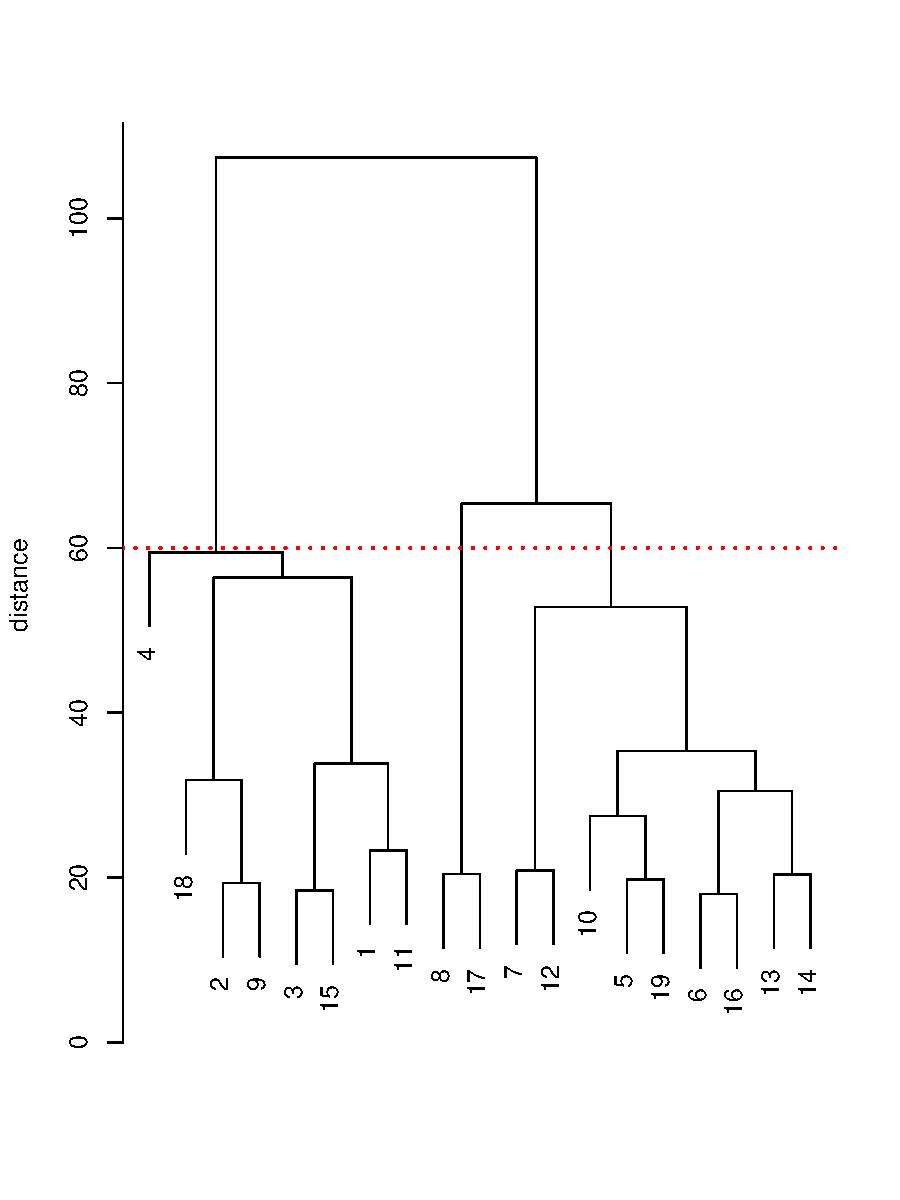
\includegraphics[width=\maxwidth]{figure/unnamed-chunk-1-1} 

\end{knitrout}
\caption{Древовидная диаграмма кластеризации ИС-Б11}
\label{fig1}

\end{figure}

\begin{figure}[H]
\centering
\begin{knitrout}
\definecolor{shadecolor}{rgb}{0.969, 0.969, 0.969}\color{fgcolor}\begin{kframe}
\begin{alltt}
\hlkwd{plot}\hlstd{(}\hlkwd{hclust}\hlstd{(}\hlkwd{dist}\hlstd{(isB12sem2[,} \hlnum{2}\hlopt{:}\hlkwd{ncol}\hlstd{(isB11sem2)])),} \hlkwc{xlab}\hlstd{=}\hlstr{""}\hlstd{,} \hlkwc{ylab}\hlstd{=} \hlstr{"distance"}\hlstd{,}
  \hlkwc{sub}\hlstd{=}\hlstr{""}\hlstd{,} \hlkwc{main}\hlstd{=}\hlkwa{NULL}\hlstd{)}
\hlkwd{abline}\hlstd{(}\hlkwc{h}\hlstd{=}\hlnum{45}\hlstd{,} \hlkwc{col}\hlstd{=}\hlstr{"red"}\hlstd{,} \hlkwc{lwd}\hlstd{=}\hlnum{2}\hlstd{,} \hlkwc{lty}\hlstd{=}\hlnum{3}\hlstd{)}
\hlkwd{abline}\hlstd{(}\hlkwc{h}\hlstd{=}\hlnum{50}\hlstd{,} \hlkwc{col}\hlstd{=}\hlstr{"red"}\hlstd{,} \hlkwc{lwd}\hlstd{=}\hlnum{2}\hlstd{,} \hlkwc{lty}\hlstd{=}\hlnum{3}\hlstd{)}
\end{alltt}
\end{kframe}
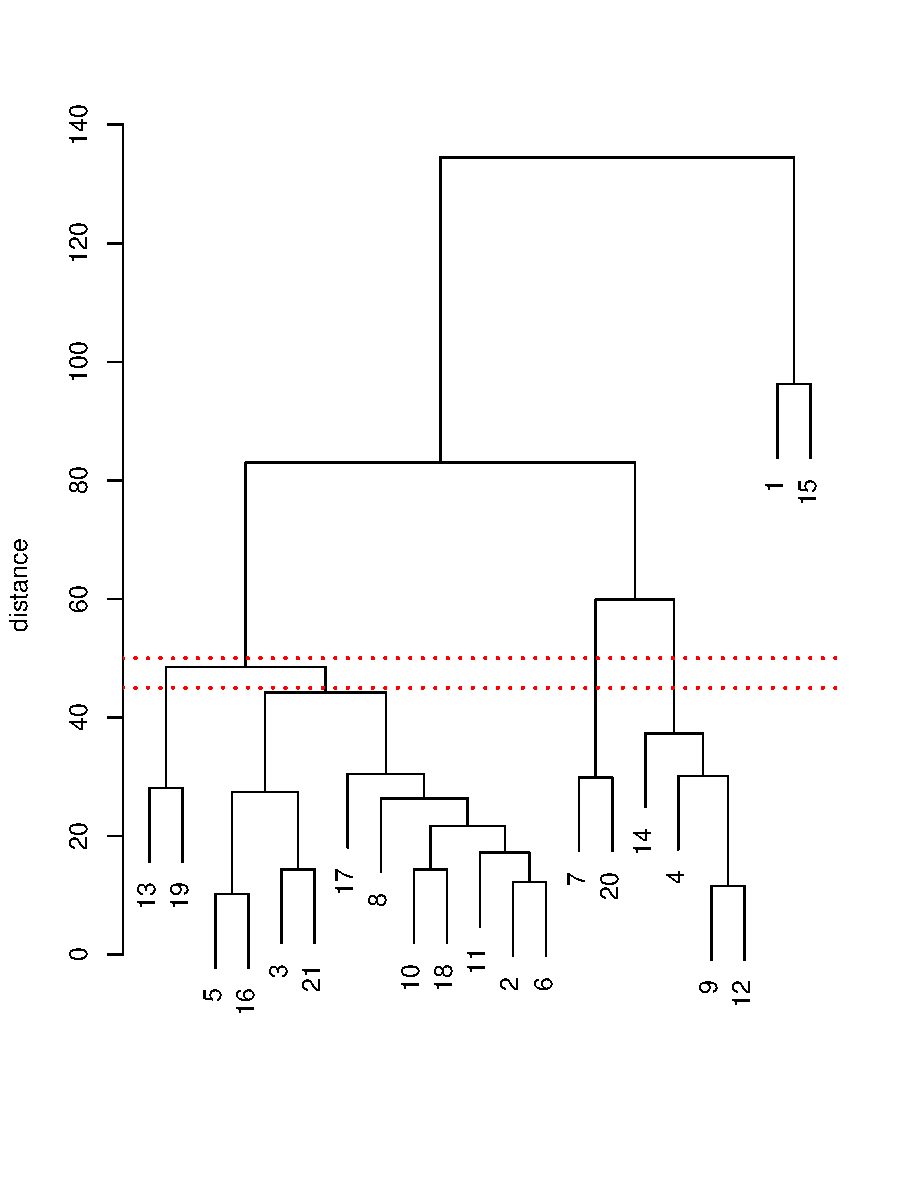
\includegraphics[width=\maxwidth]{figure/unnamed-chunk-2-1} 

\end{knitrout}
\caption{Древовидная диаграмма кластеризации ИС-Б12}
\label{fig2}

\end{figure}

\subsubsection{Выбор дисциплин для визуализации k-means}
На основании достаточно большого межквартильного размаха (IQR) были выбраны соответствующие дисциплины для визуализации результатов кластеризации по алгоритму kmeans. Таким образом, в качестве осей выбирались дисциплины с достаточно большим разбросом оценок.Дополнительно к IQR была вычислена медиана для более конкретного представления о разбросе оценок студентов.

\begin{knitrout}
\definecolor{shadecolor}{rgb}{0.969, 0.969, 0.969}\color{fgcolor}\begin{kframe}
\begin{alltt}
  \hlstd{discB11} \hlkwb{<-} \hlstd{B11} \hlopt \hlkwd{group_by}\hlstd{(discid)} \hlopt \hlkwd{summarise}\hlstd{(}\hlkwd{n}\hlstd{(),} \hlkwd{IQR}\hlstd{(sum))}
  \hlstd{discB12} \hlkwb{<-} \hlstd{B12} \hlopt \hlkwd{group_by}\hlstd{(discid)} \hlopt \hlkwd{summarise}\hlstd{(}\hlkwd{n}\hlstd{(),} \hlkwd{IQR}\hlstd{(sum))}
  \hlstd{studB11} \hlkwb{<-} \hlstd{B11} \hlopt \hlkwd{group_by}\hlstd{(stid)} \hlopt \hlkwd{summarise}\hlstd{(}\hlkwd{n}\hlstd{(),} \hlkwd{median}\hlstd{(sum))}
  \hlstd{studB12} \hlkwb{<-} \hlstd{B12} \hlopt \hlkwd{group_by}\hlstd{(stid)} \hlopt \hlkwd{summarise}\hlstd{(}\hlkwd{n}\hlstd{(),} \hlkwd{median}\hlstd{(sum))}

  \hlstd{discB11}
\end{alltt}
\begin{verbatim}
## # A tibble: 10 x 3
##    discid `n()` `IQR(sum)`
##     <int> <int>      <dbl>
##  1      2    19       17.5
##  2      3    19        3.5
##  3      6    19       22.5
##  4     12    19       15.0
##  5     14    19       12.5
##  6     23    19       20.5
##  7    171    19        0.0
##  8    339    19        0.0
##  9    913    19       10.0
## 10   1114    19       17.5
\end{verbatim}
\begin{alltt}
  \hlstd{discB12}
\end{alltt}
\begin{verbatim}
## # A tibble: 10 x 3
##    discid `n()` `IQR(sum)`
##     <int> <int>      <dbl>
##  1      2    21         15
##  2      3    21          5
##  3      4    21         10
##  4      6    21         20
##  5     12    21         13
##  6     14    21         11
##  7     21    21         20
##  8     23    21         19
##  9    171    21          0
## 10    339    21          0
\end{verbatim}
\end{kframe}
\end{knitrout}

Идентификаторы выбранных дисциплин: 6 и 23 для ИС-Б11 и 6 и 21 для ИС-Б12.

\subsubsection{Визуализация k-means}
Имена дисциплин загружаются в подпись графика динамически через функцию \verb|getDiscName(id)|

\begin{knitrout}
\definecolor{shadecolor}{rgb}{0.969, 0.969, 0.969}\color{fgcolor}\begin{kframe}
\begin{alltt}
\hlstd{getDiscName} \hlkwb{<-} \hlkwa{function}\hlstd{(}\hlkwc{id}\hlstd{) \{}
  \hlstd{name} \hlkwb{<-} \hlkwd{filter}\hlstd{(adata, discid} \hlopt{==} \hlstd{id)}
\hlkwd{return}\hlstd{(}\hlkwd{pull}\hlstd{(name, discname)[}\hlnum{1}\hlstd{])}
\hlstd{\}}
\end{alltt}
\end{kframe}
\end{knitrout}

\begin{figure}[H]
\centering

\begin{knitrout}
\definecolor{shadecolor}{rgb}{0.969, 0.969, 0.969}\color{fgcolor}\begin{kframe}
\begin{alltt}
\hlkwd{plot}\hlstd{(isB11sem2[,}\hlkwd{c}\hlstd{(}\hlstr{"6"}\hlstd{)], isB11sem2[,}\hlkwd{c}\hlstd{(}\hlstr{"23"}\hlstd{)],} \hlkwc{col}\hlstd{=k1}\hlopt{$}\hlstd{cluster,}
  \hlkwc{xlab}\hlstd{=}\hlkwd{getDiscName}\hlstd{(}\hlnum{6}\hlstd{),} \hlkwc{ylab}\hlstd{=}\hlkwd{getDiscName}\hlstd{(}\hlnum{23}\hlstd{))}
\end{alltt}
\end{kframe}
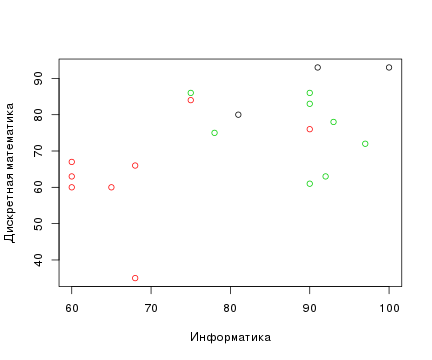
\includegraphics[width=\maxwidth]{figure/unnamed-chunk-3-1.png} 

\end{knitrout}
\caption{Результат кластеризации kmeans для ИС-Б11}
\label{fig3}
	
\end{figure}

\begin{figure}[H]
\centering
	
\begin{knitrout}
\definecolor{shadecolor}{rgb}{0.969, 0.969, 0.969}\color{fgcolor}\begin{kframe}
\begin{alltt}
\hlkwd{plot}\hlstd{(isB12sem2[,}\hlkwd{c}\hlstd{(}\hlstr{"6"}\hlstd{)], isB12sem2[,}\hlkwd{c}\hlstd{(}\hlstr{"21"}\hlstd{)],} \hlkwc{col}\hlstd{=k2}\hlopt{$}\hlstd{cluster,}
  \hlkwc{xlab}\hlstd{=}\hlkwd{getDiscName}\hlstd{(}\hlnum{6}\hlstd{),} \hlkwc{ylab}\hlstd{=}\hlkwd{getDiscName}\hlstd{(}\hlnum{21}\hlstd{))}
\end{alltt}
\end{kframe}
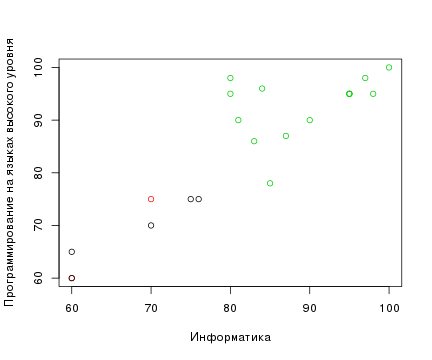
\includegraphics[width=\maxwidth]{figure/unnamed-chunk-4-1.png} 

\end{knitrout}
\caption{Результат кластеризации kmeans для ИС-Б12}
\label{fig4}
	
\end{figure}

\subsection{Статистический анализ}

\end{document}


